\documentclass[a4paper,11pt]{report}
\pdfoutput=1

\usepackage[english,swedish]{babel}
\usepackage[T1]{fontenc}
\usepackage[utf8x]{inputenc}
\usepackage{listings, babel}
\usepackage{graphicx}
\usepackage[colorlinks=true,linktoc=page]{hyperref}
\usepackage[nonumberlist]{glossaries}
\usepackage{subcaption}
\lstset{breaklines=true,basicstyle=\ttfamily}
\usepackage[margin=2cm]{geometry}
\usepackage{lipsum}

\selectlanguage{english}


\newcommand{\image}[4]{
  \begin{figure}[here]
  \centering
  \includegraphics[width=10cm]{images/#1} 
  \caption[#3]{#4}
  \label{fig:#2}
  \end{figure}
}


\title{Fault detection in photovoltaic systems}
\author{David Nilsson}

\date{May 2014}
\blurb{Master's Thesis at CSC\\Supervisor: Olov Engwall, KTH\\Examiner: Olle Bälter, KTH}
\trita{TRITA xxx yyyy-nn}

\begin{document}
\frontmatter
\pagestyle{empty}
\maketitle
\selectlanguage{english}

\input{abstract-diff.tex}

\clearpage
\tableofcontents*
\mainmatter
\pagestyle{newchap}
\pagenumbering{gobble}

\chapter*{Preface}
\addcontentsline{toc}{chapter}{Preface}
This master's thesis has been carried out during the spring of 2014 at Optistring Technologies AB in Stockholm, Sweden.
I would like to thank both of my advisors Anders Lindgren and Olov Engwall for their help throughout the project.
In addition, I would like to thank Tomas Modéer for providing invaluable feedback.
Finally I truly appreciate all support and feedback from the thesis group and colleagues at the company.

\printglossaries
\cleardoublepage
\listoffigures
\clearpage
\pagenumbering{arabic}

\chapter{Introduction}
This chapter introduces the purpose of this thesis and gives a general outline of photovoltaic systems and failure detection.
The scope and constraints are described and put into the context of the field of PV (photovoltaic) power electronics, i.e. power generation based on the sun as the energy source.

\section{Photovoltaic power generation}
Power generation based on photovoltaic sources has gradually become an increasingly larger source of power generation during the last few decades~\cite{Zhao2010thesis}.
This trend has been matched with research into more efficient solar panels.
Efficiency is measured as the ratio of incoming sun energy to the maximum attainable output power, with the current record being an efficiency of $44.7\%$~\cite{Fraunhofer2013}.
In addition to research into solar panels there is also an established interest in the surrounding equipment.

Part of these systems are power inverters converting dc energy from the solar panels to the ac grid output.
The efficiency concerns of solar panels naturally extend throughout the system, since any losses will affect the final efficiency of the complete system.
Recently the area of photovoltaic (PV) inverters has progressed to distributed systems of inverters where a small inverter module is connected to every panel~\cite{Roman2006}.
This is beneficial since each panel can be optimized locally, thereby increasing the energy harvest.
In addition to increased efficiency this also allows individual measurements of solar panels.

These new capabilities provide new possibilities in monitoring of the health of solar panels.
This process, known as fault detection, is an active research area.
Fault detection aims to detect faulty and degraded solar panels as soon as possible. 
Degradation occurs naturally in solar panels and it is of interest to quantify the degradation rate over time.

\section{Purpose of this thesis}
The purpose of this thesis is to study and develop new methods for fault detection in the context of distributed inverter systems.

\subsection*{Problem statement}
Can potential faults in a solar panel, in the context of installations with the specified properties, be detected by studying the available measurements?
This includes the capability of differentiating panel faults from partial shading of the panel.
The problem is how to perform detection efficiently in the presence of different system configurations, but also geographic and thermal dependencies, since all systems deliver different power curves.

\newpage
\subsection*{Constraints}
The most important scope limitation is that systems should only be studied passively, i.e. the available measurements are used to detect faulty panels.  
Some technical constraints are present as well:
\begin{itemize}
\item The solar panels have 60 or 72 cells built of mono- or poly-crystalline silicon
\item The installations have 14 to 24 panels connected within a small geographic area
\item The available measurements (from each panel) are:
$U$ \footnote{Panel voltage measured continuously at an optimal load},
$I$ \footnote{Panel current measured continuously at an optimal load} and
$T_{module}$ \footnote{Low resolution temperature measurement from within the PV inverter}.

\end{itemize}

This reflects the consumer market of smaller panel installations with some of the most common panel types.
The type of solar panels constrains the possible output power range and defines appropriate parameters for testing.
Due to time constraints, the simulation of solar panels has been largely based on existing data streams.
These are used as a basis of generating approximate individual panel curves, limiting the amount of effort required.

The supervising company provides data feeds providing real time measurements of several PV installations in Sweden.
This data is accumulated in a central database for further analysis and
can be used in order to verify real-life performance of a classification system, primarily to verify that working systems are not classified as faulty.

Additionally there are other sources that can be used to build realistic simulation models, such as measured solar energy over several years.
In the context of this thesis it has been assumed that access to irradiance data is available for a specific solar installation.

\section{Intended readers}
The main target audience interested in this thesis are companies building products in the field of PV power electronics.
Fault detection in solar panels is an active research area and evolves continually, demonstrating an academic interest as well.
The main party interested in the results is of course the supervising company, whom are likely to
integrate a functional solution into their final product.
While being a fairly specialized thesis, it is comprehensible to anyone with a basic background in statistics.
Some basic knowledge of physics and electronic circuits is needed as well in order to fully understand the electrical models.

\section{Sustainability considerations}
From a societal perspective this thesis has mainly a positive impact in three different ways.

The first main improvement is increased efficiency since faulty solar panels are detected and can be be replaced sooner.
This improvement has a direct benefit in total produced power.
Studies have shown there is a significant power loss due to faults in solar panels.
For example a study conducted in Britain concluded losses upwards $18.9\%$ during the first year of operation~\cite{Firth2010}.
Even though such losses would not be completely eliminated, it is reasonable to conclude that more efficient and reliable detection routines results in faster replacement of faulty panels.

Secondly, early detection of faulty panels results in fewer faulty panels being present in installations.
This results in a reduction in risk of fire hazards~\cite{Zhao2010night} which may affect both personnel and installed equipment.

Thirdly, there is a reduction in labor required for the equivalent amount of monitoring.
The final product should send alerts upon recognizing faulty panels, bypassing any manual supervision of the systems.
In the long term this implies more cost-effective installations and improved sustainability for photovoltaic systems.

\section{Methodology}
The scientific question is answered in this thesis by implementing algorithmic solutions to all the three subproblems in isolation.
This approach was taken since an empirical evaluation, subject to the unique constraints in this thesis, is the only way of surveying actual performance and applicability of different methods.
As an example of this, it is important to understand the effects of constraining the available set of measurements.
The evaluation is done by implementing a simulation framework, which is discussed in detail in the implementation chapter.

There is also a part consisting of a literature study.
This provides a deeper understanding of the field and results in a set of suitable implementation choices.
In addition, it results in a study which can be understood in the context of current research and extended upon in the future.

\chapter{Background}
This chapter introduces the concept of solar cells, including the underlying physics,
and how they work together with power inverters on the system level.
It is important to have an understanding of the underlying concepts when discussing the applicability of different methods to failure detection.
These concepts are however generic and common knowledge in the field of PV power generation, 
hence this chapter can be skipped given a sufficient existing background.

\section{Theory of the solar cell}
Solar cell technology can be broadly described as equipment converting incoming photons (typically sunlight) to electric energy.
The solar cells of interest in this study are mono- and poly-crystalline silicon, technologies that currently have a large market share~\cite{Zhao2010thesis}.

Both of these share the property of being being constructed around a single pn-junction, i.e. the connection between two differently doped silicon areas.
The incoming photons may be absorbed by the silicon in which case a electron-hole pair is created~\cite{Zhao2010thesis}, since the electron is pushed to an outer layer by the absorbed energy.
Connecting an electric load, such as a heating element, to the terminals of the solar cell will then induce a direct current.
Overall this results in an efficiency of $13-18\%$ for single-junction silicon technology~\cite{Zhao2010thesis}.

The solar cell can by analyzed using an equivalent electrical circuit model with well-defined parameters.
A broadly used model is the one-diode model~\cite{Walker2001} as shown in figure \ref{fig:solar-cell-equiv}.
It is based on modelling the solar cell as a current source connected in parallel with a diode.
In addition there are inherent losses due to imperfect manufacturing.
These are modelled as a series and a parallel resistance.
The resulting current $I_{load}$ flows across the terminals through a load with potential difference (voltage) $U_{load}$.
$I_{photo}$ corresponds to the amount of current generated by incoming photons which is proportional to the irradiance and area of the solar cell.

\begin{figure}[!ht]
\centering
\begin{subfigure}{0.4\textwidth}
  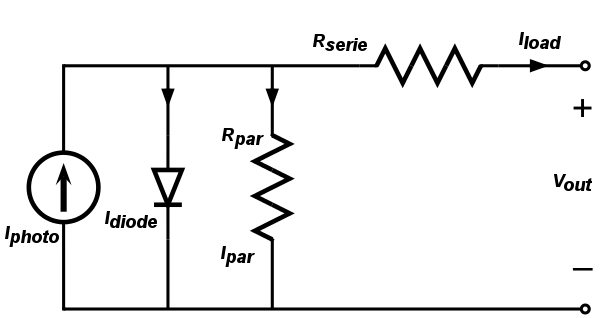
\includegraphics[width=\linewidth]{solar-cell-equiv.png}
\end{subfigure}
~
\begin{subfigure}{0.4\textwidth}
  \begin{tabular}[b]{| c | c |}
  \hline
  $I_{load}$ & load current \\ \hline
  $U_{load}$ & load voltage\\ \hline
  $I_{photo}$ & photogenerated current \\ \hline
  $I_{diode}$ & diode current \\ \hline
  $I_{par}$ & parallel loss current \\ \hline
  $R_{par}$ & parallel loss resistance \\ \hline
  $R_{serie}$ & series loss resistance \\ \hline
  \end{tabular}
\end{subfigure}
  \caption[Equivalent circuit of a solar cell]{
    \emph{
    Equivalent circuit of a solar cell based on a current source and diode,
    with losses represented by a series and a parallel resistance.
    The table describes all variables of the one-diode model.
    }
  }
  \label{fig:solar-cell-equiv}
\end{figure}

\clearpage
The model can be formalized in order to solve for the resulting current and voltage, given the parameters of a solar cell.
Summing up all the currents it holds that $I_{photo} = I_{diode} + I_{par} + I_{load}$.
Using the well known Ohm's law followed by Shockley's diode equation~\cite{Walker2001}, the following holds:

\begin{multline}
\label{eq:eq-circuit}
I_{load} = \\
I_{photo} - I_{diode} - I_{par} = \\
I_{photo} - I_{diode} - \frac{R_{serie}I_{load} + U_{load}}{R_{par}} = \\
I_{photo} - I_{sat}(e^\frac{q(R_{serie}I_{load} + U_{load})}{k_B T} - 1) - \frac{R_{serie}I_{load} + U_{load}}{R_{par}}
\end{multline}

$I_{sat}$ denotes the constant saturation current of the diode,
$k_B \approx \SI{1.38e-23}{\joule\per\kelvin}$,
and $q \approx \SI{1.60e-19}{\coulomb}$.

The free variables are $I_{load}$, $U_{load}$ and $T$, where $T$ is the temperature measured at the p-n junction.
All parameters of the model, such as $I_{sat}$, may be given in a datasheet or can alternatively be extracted by performing non-linear regression based on samples of the free variables~\cite{Walker2001}.

There are several relevant aspects in understanding this equivalent model when performing analysis of power generated from solar panels.
Firstly the output current is proportional to the incoming irradiance, which directly affects $I_{photo}$.
Figure $\ref{fig:trina-iv-curve}$ shows a plot of $I_{load}$ as a function of $U_{load}$ at different irradiations.
The panel is held at a constant temperature.

\image{trina-60cell-iv-alpha.png}{trina-iv-curve}{Solar panel I-V curve characteristic}{
  Typical I-V curve of a solar panel. Note the non-linear relationship between voltage and current, and the effect of solar irradiation on output current.
}

In addition to changing irradiation there might also be a range of operating temperatures depending on local weather conditions.
The temperature affects the second term in equation \ref{eq:eq-circuit} and increased temperature results in decreased load current.
This is important to take into account since otherwise increased temperature might be mistaken for decreased irradiation.
While being an important source of measurements in general, this study only concerns fault detection based on samples of $I_{load}$ and $U_{load}$, but still needs to perform reliable classification.

Finally, it is important to realise that different solar panels have different parameters and will yield different I-V curves.
This implies that inhomogeneous systems offer challenges when comparing produced power output, for example in the case of fault detection.

\section{Systems of solar panels}
Single solar cells of the types described previously typically generate an output voltage of \SIrange{0.6}{0.7}{\volt}~\cite{Zhao2010thesis}.
A solar module connects several solar cells and places them into a rigid enclosure.
This module can then be mounted as part of a larger system.
Figure \ref{fig:solar-module-generic} shows a 54-cell module with the output dc terminals visible on the backside.

\image{solar-module-generic.jpg}{solar-module-generic}{Generic solar module}{
  Back and front of a generic 54-cell silicon solar module. Every cell and the vertical interconnections are clearly visible.
}

In addition to protecting the fragile silicon sheets, the purpose of the module is also to improve yield by using an anti-reflective coating.
This thesis considers modules containing 60 or 72 solar cells of the previously specified type, connected in series.
The resulting I-V curve of the module has an increased width and every point is stretched to $n \cdot U_{load}$ with $n$ cells each producing at some $U_{load}$.

There is however also some extra components involved in the module circuitry.
The panel is divided into y substrings of which each has a diode connected in parallel.
During normal operation the diodes will not carry any current.
If some cell is reduced in performance, for example by having an unusually high series resistance, this will result in the corresponding diode conducting the current, effectively bypassing that specific substring~\cite{Roman2006}.
This is relevant since the I-V curve will reflect these properties and should be analyzed while keeping these effects in mind.

\section{The role of PV inverters}
Solar panels produce direct current as previously described.
This is suitable for certain types of applications such as charging batteries.
It is however not suitable for generation on the electric grid which uses ac power at a fixed voltage.
This conversion is done using a power inverter, also known as PV inverter.
There are different topologies applicable, i.e. different arrangements of both solar panels and PV inverters.
Traditionally a common configuration has been to use long strings of modules connected in series with a single big inverter at the end of the string.
This approach is, however, constrained due to individual modules having an unproportional influence on the total power yield of the string~\cite{Roman2006}.

\image{optistring-inverter.jpg}{optistring-inverter}{Optistring PV inverter}{
  The distributed Optistring PV inverter with dc input and ac output.
  A separate inverter is placed on the back of every solar panel.
}

The system considered in this study is a distributed version with a typical inverter shown in figure \ref{fig:optistring-inverter}.
Each module has its own simple PV inverter acting as an independent ac power source.
In addition to providing higher efficiency, this also produces $I_{load}$ and $U_{load}$ measurements from every individual module.
This is highly relevant since studies in fault detection typically consider a specific topology and the results might not always generalize to the distributed case.

A PV inverter should transform the power in the most efficient way and more specifically ensure that the panel is being applied to an optimal load.
This corresponds to finding the point on the I-V curve where $I_{load} \cdot U_{load}$ is maximal, which is known as the maximum power point (MPP).
Examples of search methods include Pertube and Observe and Incremental Conductance~\cite{Roman2006}.
These are relevant to this study since local searches may not be well-behaved during panel faults~\cite{Roman2006}.
This is due to the existence of multiple local maxima on the I-V curve, resulting in the possibility of considering a local optima as a global maxima.
Previous studies have also found that MPP tracking (MPPT) might prevent faults from being observed during night-to-day transitions~\cite{Zhao2010night}.

A relevant term applicable to measuring the efficiency of solar cells is \emph{fill factor} which is defined as the ratio between the power at $I_{MPP} \cdot U_{MPP}$ and $I_{max} \cdot U_{max}$.
The maximum reference values are defined as $I_{max}$ being the current measured in closed circuit and $U_{max}$ being the voltage measured without any load connected.


\section{Solar power in practice}
Given an understanding of the different components of a PV solar installation it is also important to reflect on real-life behaviour.
The power output of an installation and individual solar panels vary to a large degree.
Figure \ref{fig:january-power-curve} and \ref{fig:october-power-curve} illustrate this, where a 10-fold decrease in peak power output is seen over a period of 3 months.
In addition the total duration of power output is reduced by 4 hours.
Another interesting aspect of these graphs is the significant amount of noise present due to shadowing.

\begin{figure}[here]
\centering
\subimage{january-power-curve.png}{january-power-curve}{TBD}{
   Power curve captured during a day in January 2014.
}{0.48}
~
\subimage{october-power-curve.png}{october-power-curve}{TBD}{
  Power curve captured during in a day in October 2013. Note the use of a different scale on the Y-axis.
}{0.48}
\caption[Power curves captured from an installation]{\emph{Power curves (in Watt) captured from a 16-module installation based in Stockholm, Sweden.}}
\end{figure}

After sunset and during periods of negligible irradiance the system is completely shutdown.
This is done in order to reduce power consumption and thereby increase overall efficiency.
In addition to seasonal and geographical dependencies, the power output is also proportional to the number of solar panels in the system and affected by the type of each panel.
All of these highly varying conditions impose restrictions on how fault detection can be implemented and the required scope of validation.
The main point is that developed methods need to be dynamic and adaptive to any applicable system configuration.

\chapter{Theory of fault detection}
Based on knowledge of how a PV system produces energy and the underlying dependencies,
it is possible to reason about faults.
Faults in PV systems can be characterized as permanent power losses but a more fine-grained analysis might be suitable if there are failure-specific patterns that can be utilized.
This chapter gives an overview of possible failure conditions and describes the different kinds of methods that have been established by previous studies.

\section{Issues in photovoltaic systems}
There are a lot of studies analyzing different issues present in PV systems \cite{Baltus1997,King2002,Petrone2008}, demonstrating an interest in detecting faults to the greatest extent as early as possible.

A study conducted in Spain~\cite{Munoz2011} discusses the following failures in solar modules:
\begin{itemize}
\item Yellowing and browning
\item Delamination
\item Bubbles in the solar module
\item Cracks in cells
\item Defects in anti-reflective coating
\item Hot spots caused by the panel acting as a load
\end{itemize}

Another study~\cite{Forman1982} identified the following conditions:
\begin{itemize}
\item Edge-seal delamination
\item Newly cracked cells
\item Delamination over cells and interconnections
\item Split encapsulation over cells and interconnections
\item Protruding interconnections
\end{itemize}

It has also been found that connections and the welds can degrade over time \cite{Houssein2010}.

In conclusion it can be said that there is a wide range of failure conditions.
This breadth motivates the use of classes of failures, based on the electrical properties induced during a fault.
\cite{Zhao2010thesis} and the papers \cite{Zhao2012tree,Zhao2013graph,Zhao2013outlier} use a categorization into ground faults, line-line faults, and open-circuit faults.
Ground faults are defined as a conductor accidentally having contact with the system ground~\cite{Zhao2010thesis}.
Line-line faults occur when two different potentials conduct by accident~\cite{Zhao2010thesis}.
Open-circuit faults occur when a conductor is accidentally removed from a closed circuit~\cite{Zhao2010thesis}.
The same study concludes that ground and line-line faults typically exhibit a significant drop in output voltage,
but also states that open-circuit faults and degradation causes significant decrease in current.

The same thesis found that protection devices commonly present in PV installations known as over-current protection devices (OCPD) and ground protection (GPD) are not sufficient.
During certain kinds of faults the MPPT may interfere and lower the current output, which in turn will not trigger the current-based protection devices.
Similar issues are present when faults occur during the night \cite{Zhao2010night}.

In the context of degradation over time it has been found that dust is a significant problem \cite{Mani2010}.
These effects are however very dependent on the geographical position and the physical alignment with respect to weather conditions.

A study \cite{Munoz2011} found that early degradation occurs due to wide variety for reasons.
The paper ties the measured degradation rates to a specific allowance, based on guarantees from the manufacturer.
It discusses a typical guarantee of $90\%$ over 10-15 years and $80\%$ over 20-25 years with preserved nominal power.

Meyer and Dyk~\cite{Meyer2004} note that degradation in the anti-reflective coating results in a brightening in the color of the cell.
It can also be detected in the module's maximum attainable voltage and current.
The paper discusses solar cell degradation as three different factors being involved in relation to the one-diode model figure \ref{fig:solar-cell-equiv}.
The first is an increase in series resistance, the second is a decrease in the parallel resistance (which implies a larger loss current), and the third being deterioration of the anti-reflection coating affecting the photogenerated current.

Concrete percentual figures of degradation have also been studied~\cite{Quintana2002}, which cites a degradation rate of about $0.7\%$ per year for multi-crystalline modules.
There is also a note on that the system may continue to operate in degraded conditions without causing an intermediate failure.
The paper also describes a condition known as \emph{light induced degradation} (LID) which is a module degradation
that occurs once during the first few hours of sunlight exposure.
It is stated that at most a $5\%$ degradation in maximum attainable current has been observed.

\section{Partial shading of solar panels}
Partial shading occurs when a subset of the PV array is shaded to some degree.
This occurs naturally for example due to passing clouds.
Nearby obstacles might also interfere and cast shadows, resulting in reduced power output.
Hence, shading conditions is a relevant aspect when planning a PV installation.
Due to the nature of the resulting power reduction it is also relevant to classify power output into either the case of partial shading or faulty panels.

Some studies, e.g. \cite{Stettler2005}, view partial shading as another failure condition.
This somewhat simpler view does not require partial shading to be separated from for example faulty solar panels.

Partial shading has been studied in isolation \cite{Alsayid2013}.
The paper illustrates the effect of bypass diodes triggered due to shadow conditions, resulting in non-smooth I-V curves with different characteristics.
However, it does not describe suitable classification attributes or relate shading to fault conditions.
The results are also heavily dependent on the panel topology and placement of bypass diodes.

A study based on measurements in the UK \cite{Firth2010} considers classification of faults as partial shading.
The approach taken is to, based on the position of the sun, measure the frequency of errors at individual segments in the solar plane.
The solar plane is viewed as solar elevation on the y axis and solar azimuth on the x axis.
Small 5-minute segments of this plane are then considered in isolation.
A fault is considered as partial shading if the frequency of faults in the corresponding segment is higher than an experimentally calculated threshold.
The actual frequency is simply calculated as the number of failure-free occurrences of the segment with respect to the number of faults within the segment.

\clearpage
\section{Approaches to fault detection}
A basic approach to detecting unexpected power loss is comparing the output with a reference value and triggering an alarm when large differences are detected.
The approach taken in~\cite{Stettler2005} is to perform monitoring using satellites, essentially building up known weather conditions.
This approach is not applicable to this study due to insufficient weather data available.

An extension of this method is building an analytical model \cite{Chouder2010,Raina2013,Chao2008}
based on the one-diode model introduced previously (equation \ref{eq:eq-circuit}).
All parameters are retrieved from the manufacturers datasheet or through parameter extraction \cite{Eicker2005,Chouder2009,Walker2001}.
This method relies on access to both irradiance and solar panel temperature measurements in order to calculate the reference MPP.
This is then compared to the measured working point as previously discussed.

An active approach is described in \cite{Meyer2004}, where the whole I-V curve is studied for defects, and the maximum attainable $U_{max}$ and $I_{max}$ are recorded over time.
Due to the nature of sweeping I-V curves this implies that this gives a reduction in power output during the analysis.
In addition it is not applicable to passive studies of systems since they can be assumed to deliver output at MPP.

Two studies by Vergura et al.~\cite{Vergura2008,Vergura2009} consider several identical PV strings and compare the outputs in order to classify significant deviations.
This is done by checking if certain statistical assumptions can be made, formally that the power differences are independently normally distributed with identical variance.
If this is the case, a method known as analysis of variance (ANOVA)~\cite{Vergura2009} can be applied in order to build confidence interval for the power output of each PV string.
Otherwise the Kurskal-Wallis test~\cite{Vergura2009} is applied in order to build the corresponding intervals.
The resulting confidence intervals can be studied for significant deviations which would imply defect solar modules.
While not being directly applicable to this study, the papers remain relevant due to the basic assumption of only having access to power measurements.

Another statistical approach is taken by Zhao~\cite{Zhao2013outlier} that is centered around outlier detection.
Similarly to \cite{Vergura2008,Vergura2009}, the Zhao paper assumes a set of identical PV strings and tries to classify deviations.
This is done by building confidence intervals using three different methods: 3-Sigma rule, Hampel identifier, and Boxplot rule.
All of the surveyed methods exhibit different properties, but the paper concludes that the Hampel identifier and Boxplot rule are suitable for fault detection.
Based on the assumptions made, the paper can consider all PV string currents as samples taken from a single normal distribution, allowing straight-forward statistical analysis.
This simplification is however not directly applicable to this study.

In the case of given knowledge surrounding faults it is possible to apply supervised learning, e.g. \cite{Zhao2012tree},
where a labelled dataset is available containing measurements classified manually.
This dataset can for example be generated by measuring voltage and current of solar modules while injecting faults.
The paper discusses a decision tree model that takes the available measurements and locates the most probable classification based on the dataset.
Classification performance is concluded to be very good but real-life applications are limited due to the dataset being heavily tied to a specific PV installation.

A natural extension is analyzed in \cite{Zhao2013graph} which considers the case of graph-based semi-supervised learning, where only a small amount of reference data is available from the start.
This approach results in significant cost reductions, due to the low amount of labeled data, but is also possible to adapt to changing conditions in different systems.
The classification performance is up to $99\%$ for certain classes of errors.

Finally, \cite{Kang2012} takes the approach of using a Kalman filter in order to predict power output.
The Kalman filter~\cite{Kang2012} takes a set of noisy measurements and the underlying physical model, and produces the most probable output value in an iterative process.
This is used in order to locate faults based on measurements of voltage, current, and panel temperature.
Notably this permits classification without access to irradiance data.
The requirement of access to to panel temperature is however limiting in the context of this report.

There has also been research into locating the faulty panel within a string~\cite{Lin2012}.
These results can be considered less applicable when individual solar module measurements are available.

\section{Measuring degradation}
Panel degradation needs to be measured in order to quantify the losses due to possible faulty panels that may void any established guarantee conditions.
Traditionally several different manual techniques have been utilized~\cite{Munoz2011} such as IR-based camera snapshots, exposure to strong light, and I–V curve analysis string by string.

The PVSAT project~\cite{Stettler2005} considers faults based on their long-term effects.
Losses are classified as panel degradation after a long period of time has passed with an energy reduction in the range of $0-20\%$.

A recent master's thesis~\cite{Zhao2010thesis} simulates degradation in order to test the implemented methods.
In this model a variable series resistance is introduced in the solar module.
The resistance is then gradually increased over time in order to provide a significant decrease.
This loss corresponds to $R_{serie}$ in the one-diode model (figure \ref{fig:solar-cell-equiv}).

One approach to detecting degradation is measuring the fill-factor over time~\cite{Raina2013}.
The fill factor is calculated by approximating the maximum attainable current and voltage through parameter estimation.
The cited study is however constrained to installations with measurements of irradiance and temperature, and hence not applicable to this report.

Finally, \cite{Makrides2010} evaluates degradation over longer time periods by using several techniques.
The study assumes access to irradiation and temperature and samples the produced power during periods of high irradiance.
All measurements are normalized by considering both the irradiance and temperature conditions.
These values are then averaged on a monthly basis using a least squares method.
Annual degradation can then be quantified by comparing months pairwise over a year.
The study makes an important remark regarding changing conditions during individual days, where all considered panel technologies suffered output losses as the day progressed.
This is attributed to changing spectral conditions.

\section{Summary}
The constraints of this thesis also affect the applicability of many of the previously mentioned methods.
Firstly, the constraint of only having access to voltage, current, and low-precision temperature values restricts the immediate applicability of many methods.
The lack of irradiance measurements contributes to a more general setting in the case of the one-diode model, since the $I_{photo}$ value needs to be considered unknown.
Since the temperature is not measured at the PN-junction, the corresponding term in the one-diode model needs to be modelled as an expression of the actual measured value.
In general this contributes to a very general theoretical model which not necessarily can be fitted onto a set of data samples, as described in studies based on an analytical model.

Secondly, it is important to distinguish between the cases of having several identical PV strings or panels, from the case of several panels with possibly different characteristics.
This implies that the methods based on outlier detection do not transfer naturally, since the offsets between panels need be taken into account.

Detection of partial shading does not have the same dependency on specifics on the solar installation, since it only assumes access to an existing flow of fault classifications.
The method of studying a solar plane and correlations with the reported faults is suitable for this thesis.

Degradation measurements are also affected by the lack of irradiation and junction-level temperature measurements.
The studies mentioned rely on correcting for these factors when comparing two points in time, in order to determine the degradation in power output.
Hence another approach would be to generalize this procedure for the case unknown irradiance and a model of the junction-level temperature.

\chapter{Implementation}
This chapter describes the approaches that have been taken to solve the problems stated in the introduction.
Each section is described separately with algorithmic outlines and general comments regarding applicability within the scope of this thesis.

\section{Simulation framework}
A central part of this thesis has been to develop a simulation framework in order to study the different problems in various aspects.
This is necessary since an algorithmic approach to e.g. fault detection needs to be evaluated under real life conditions.
It is also important to take different system characteristics and system configurations into account when presenting classification results.

% TODO Refactor description on data generation and enhance ENHANCE ENHAAAAAAAANCE
The implemented simulation framework consists of several parts.
It is implemented as a driver program which interfaces towards a database, either generating data or fetching data for e.g. classification purposes.
Data generation has been implemented based on real life measurements of yearly irradiance and temperature values gathered at a location in Stockholm, Sweden.
These inputs are used together with the parameters of a solar installation in order to generate a resulting series of voltage, current, and temperature values at 5 minute intervals.

The second part of the data generation is injecting faults into outputs from solar installations.
This has been implemented as a fault occurring at some fixed point in time, with an independent percentage loss in voltage and current.
These faults may also occur during night or during low irradiance conditions, as motivated by the possible classification difficulties previously discussed.

The generated data has then been used in order to determine classification performance.
This has been implemented as some external procedure receiving input measurements from a whole installation over time.
Hence this approach reflects real life use cases where online classification is performed.
Repeating this process over many different systems with different configurations results in statistically significant results, applicable to systems concerned in this thesis.
The procedures being applied on the data streams are described in the following sections.

\section{Immediate failure detection}
Immediate failure detection is about detecting fast degradation occurring in solar panels.
This involves both analysis of current and voltage components, motivated by the different effects being observed, as discussed in the literature study.

In this study the individual solar panels within a single installation may have different characteristics and the number of panels varies as well.
This implies that simply comparing individual panels within a system will not produce meaningful results, since large differences may correspond to the expected case during normal operation.

These properties motivate the use of a more generalized algorithm capable of handling these differences while still detecting faults reliably.
The approach taken in this study is to process individual solar panel measurement vectors, followed by iterating over increasing points in time.
This iterative procedure compares differences between solar panel outputs within the system and large differences indicate that a fault has been discovered.

This solution to immediate failure detection was chosen in order to capture the fundamental aspect of comparing differences within a single installation.
Processing samples by iterating in time allows an online-style implementation which takes as input the latest measurements and decides if a fault is found, repeatedly.
The functions outlined in the upcoming sections do not employ any kind of hypothesis testing which would potentially result in better accuracy.
Instead the focus was on developing the fundamentals of immediate failure detection, allowing future work to be focused on these improvements.

The first step of the computation is to do preprocessing of the raw measurements.
This whole process is repeated separately with current and voltage vectors.
Since there are natural variations between solar panels within a single installation, it is of interest to remove differences to ease classification of the output data.
The approach taken here is to subtract the mean and scale measurements with a measure of standard deviation.

\begin{figure}[H]
\begin{verbatim}
# Scale input matrix where rows belong to a specifc panel
scale(matrix):
  cols = matrix.cols()
  rows = matrix.rows()

  for t = 1..cols
    for panel = 1..rows
      column = matrix[1..rows][t]
      matrix[panel][t] = (matrix[panel][t] - average(column)) / std(column)
\end{verbatim}
\end{figure}

As outlined above, this process is performed over a matrix where each row corresponds to a measurement vector of a single solar panel.
Each entry is adjusted by using the corresponding column of samples corresponding to a specific point in time.

The next step of the algorithm is to filter the data series, only keeping samples taken during high irradiance.
Samples taken during the night are naturally ignored, but this also applies to samples taken during periods of very low output power.

\begin{figure}[H]
\begin{verbatim}
# Build chunks of samples based on power data
chunkSamples(scaled, power):
  chunks = []
  current = []

  for i = 1..scaled.length
    if power[i] >= POWER_THRESHOLD
      current.add(scaled[i])
    else if current != []
      chunks.add(current)
      current = []

  return chunks
\end{verbatim}
\end{figure}

The algorithm outlined above takes as input measurements from a single solar panel, with the first argument being either a current or voltage vector, and the second being the output power.
Evaluating this results in a list of consecutive periods of significant output power, each of which can be analyzed in isolation.
The constant \emph{POWER\_THRESHOLD} should be chosen accordingly, typically to about $50 W$.

Using these continuous series of samples it is possible to define the main routine which is responsible of detecting faults.
Given that faults may occur during periods of no irradiance there is a need to connect the analysis between isolated segments.
This is done by maintaining a \emph{reference window} which corresponds to the last valid point of data.
During the first segment this window is initialized in a special way.

\begin{figure}[H]
\begin{verbatim}
# Process a scaled vector of measurements
processPanel(scaled, window):
  if window not initialized
    window = average(slice(scaled, 1, windowSize))

  faults = {}
  idx = windowSize/2
  while idx <= (idx.length - WINDOW_SIZE/2 - 1)
    newRef = average(slice(scaled, idx - windowSize + 1, idx))
    sample = average(slice(scaled, idx                 , idx + windowSize - 1))

    if |window - sample| <= EPSILON
      faults.add(idx)

    window = newRef
    idx = idx + 1

  return faults
\end{verbatim}
\end{figure}

The function outlined above is responsible of locating any faults associated with a given panel during one segment of continuous measurements.
Using the previously scaled and chunked vector, \emph{processPanel} is called repeatedly on these inputs in order to gather all the located faults.
This routine performs the actual detection by comparing the reference window with a new sample window in order to detect large differences.
The code requires a function \emph{average} which computes the mean of its argument, and a function \emph{slice} which extracts the subvector indicated by the given indices.
Note the use of two constants \emph{EPSILON} and \emph{WINDOW\_SIZE}.
These correspond to the sensitivity to noise and the tolerance to fast changes in power output.
Typically a reasonable value of 16 was found for the window size, given that samples are taken at 5-minute intervals.
The other parameter required empirical testing in order to extract a reasonable value, which is discussed more in depth in the results section.

\section{Measuring degradation}
Degradation measurements are about quantifying the loss in performance over a given time period for solar panels.
As concluded in the literature study, there are no feasible methods in the context of this project.

\subsubsection{Theoretical model}
One approach utilized in several studies is to fit solar panel parameters using an equivalent electrical method.
The one-diode model can be applied onto measurements on the free variables in order to find the corresponding parameters.
These variables are irradiation-induced current, panel voltage, temperature, and panel current.
In order to apply this model to the context of this project, the loss of accurate temperature samples and unavailability of
$I_{photo}$ need to be taken into account.

Evaluation of this method was done by performing a model fit given one day's worth of data from a single panel.
In order to handle the missing $I_{photo}$ samples, it was assumed that this value was constant, known as $k$.
This implies that $k$ becomes a new variable in the model which needs to be solved for.
In addition, all input temperature measurements were of the actual panel temperature.
The results will then only establish a upper bound in performance for this method.

The resulting model together with the measurements of voltage, current, and panel temperature, were then used to estimate parameters.
This regression can be evaluated using some non-linear regression algorithm.
MATLAB implements \emph{Trust-Region-Reflective optimization} \footnote{http://www.mathworks.se/help/optim/ug/lsqnonlin.html} which is the only algorithm to support bounded variables, i.e. some variable in the model is restricted to only take on values within a certain interval.
Several runs were performed in order to evaluate this method together with bounded variable intervals established in the project constraints.
This resulted in a wide range of local minima i.e. no true set of assignments were found to the solar panel parameters.

Due to the difficulties in non-linear regression and computational constraints, this method was concluded to not be applicable.

\subsubsection{Alternative approach}
Due to the negative results involving a theoretical model it was deemed suitable to study alternative approaches to measuring degradation.
Such an approach is to place focus on detecting differences in measurements, when comparing two different points in time of the same solar installation.
Some of the studied papers in the background section included similar techniques where samples are taken only at known positions in time, for example at the peak of a normal distribution.
These do however require scaling or normalization based on unavailable parameters such as accurate panel temperature.

A generalization is to base the selection criteria on overall similarity in the measured parameters.
For example, consider the case of a solar installation being subject of nearly identical irradiation during two consecutive days.
Given that environment temperature remains similar this will lead to very similar samples being taken along the curves of both days.
The basic idea is then to generalize this concept to locating similar points in time and do a pairwise comparison in order to determine the amount of degradation that has occurred.
Note that this method is limited to only measuring relative degradation among panels, and accurate absolute measurements require that only a few panels are degraded.

Formally, the method is outlined in the following algorithmic description.

\begin{figure}[H]
\begin{verbatim}
# Count the number of valid panel samples at two points fixed in time
countValid(s1, s2, n):
  valid = 0
  for panel = 1..n
    if(|s1[panel].voltage - s2[panel].voltage|         <= VOLTAGE_EPSILON &&
       |s1[panel].current - s2[panel].current|         <= CURRENT_EPSILON &&
       |s1[panel].temperature - s2[panel].temperature| <= TEMP_EPSILON
      )
      valid = valid + 1

  return valid

# Locate all valid pairs of samples
locateSamples(firstDay, lastDay, n, k):
  # Retrieve two months worth of vector, current, and temperature vectors
  first <- fetchMonth(firstDay)
  last <- fetchMonth(lastDay)
  results = {}

  # Iterate over all (voltage, current, temperature) vectors in time
  for s1 in first
    for s2 in last
      if countValid(s1, s2, n) >= n - k
        results.add((s1, s2))

  return results
\end{verbatim}
\end{figure}

The function \emph{locateSamples} accepts two input dates, which determine the time periods of interest.
Each date describes the start of the corresponding month being swept for valid data points.
The final two parameters are the number of solar panels $n$ and the maximum number of faulty panels $k$.
The algorithm then locates any two data points in time which do not differ to a large extent.
This is defined as the voltage, current, and temperature taking values within specific threshold values.
These threshold values are denoted \emph{VOLTAGE\_EPSILON}, \emph{CURRENT\_EPSILON}, and \emph{TEMP\_EPSILON}.

The output from the algorithm above is a vector of pairs that describe matching positions in time.
Hence the this vector can be analyzed in order to draw conclusions regarding changes in the measurements taken.
In order to produce stable degradation measurements it is suitable to average all of registered samples.

The threshold values affect the precision in the returned samples.
Smaller threshold values will produce more accurate comparisons but has the inherent limitation of limiting the number of data points retrieved, eventually resulting in no data points.
Larger values are needed during time periods where solar irradiance and panel temperature varies to a larger extent, limiting the usefulness of this method in those situations.

The maximum number of faulty panels, $k$, should be set relatively small since larger values increases the probability of noisy data producing valid pairs.
This also implies a restriction in usefulness since only a limited number of degradations can be measured.

\section{Detection of partial shading}
Partial shading of solar panels occur when some obstruction limits the amount of irradiance received by the solar panels.
One method was suggested by the literature study, based on measuring the failure frequency in segments in the solar plane.

The fundamental approach of making observations in the solar plane is reasonable since shading is likely to be correlated with the sun position.
A similar approach has been taken in this project.
Using the immediate failure detection routine outlined above, any faults occurring in an installation can be recorded over time.
By using the geographical position of the installation, and the timestamp of the fault, the corresponding solar position can be derived.
The solar position is typically given as two angles known as azimuth and zenith.
An example of the solar plane is shown in figure \ref{fig:solar-plane-plot}.

\image{solar-plane}{solar-plane-plot}{Solar plane density plot}{
  Density plot of the solar plane during one year with brighter areas having more occurrences.
}

The figure has been created by plotting all solar paths during a year of operation of a system in Stockholm, Sweden.
Brighter areas have a higher density solar occurrences.
Hence this figure demonstrates a non-uniform distribution of paths in the solar plane.

Given the positions of all faults in the solar plane it is then of interest to partition them into real faults and partial shading occurrences.
The approach taking here is study clusters of faults.
By the previous argument it is reasonable that clustered indications were caused by the same shading.
In order to identify clusters it is suitable to use a clustering algorithm.
The DBSCAN algorithm \cite{Birant2007} is capable of locating clusters in a set of data points.
Its application to this study is motivated by the fact that it is capable of finding non-convex clusters, which may occur in the solar plane.
DBSCAN accepts two input parameters and the input vector of positions in $R^2$.
The first one is $\epsilon$ which describes the minimum distance between to points in the same cluster.
The second one is $minPts$, the minimum number of points in some cluster.
All points that are not found to be part of any clusters are classified as noise.

Using DBSCAN as a clustering algorithm implies a new problem, namely parameter selection.
Due to the nature of clustering there is not a given set of parameters that fit all problems.
In this study it was found that $\epsilon = 8$ and $minPts = 3$ were suitable for a window of 5 days.
These values are however likely to be dependent on system configurations and specific installations.
In a real-world installation these issues can be dealt with by establishing a baseline of fault frequencies.
This would require an initial period were only shading occurred.
The parameters would then be set in such a way that all points belong to some cluster.
An alternative approach would be to limit the method to the cases where several years worth of fault occurrences have been recorded.
Given that the baseline of real faults is sufficiently low it would then be possible to locate all major clusters.

There are however some inherent issues with detecting partial shading.
Firstly, real faults may mistakenly be classified to belong to a cluster of shading faults.
Another issue is that there is a non-uniform distribution of faults in the solar plane.
Since the underlying failure detection algorithm will only report failures during non-negligible periods
of irradiance, there will be a bias with more faults during the morning.
Finally, as demonstrated by figure \ref{fig:solar-plane-plot}, the non-uniform distribution of solar paths imply that 
faults are more likely to be clustered along the outer edges.

\chapter{Results}
This chapter describes the results retrieved using the implemented methods with visualizations of classification rate and other performance measures.

\section{Immediate failure detection}
Immediate failure detection was implemented using the algorithm previously described.
Using the simulation framework, the implementation was evaluated over a wide range of system configurations.
A total of 50 different installations were randomly generated and 2000 faults were injected into these.
Each fault consists of a gradual percentual degradation in both current and voltage, and may occur during periods of no irradiance.

The classification performance can then be derived by detecting the subset of faults that are properly recognised using the algorithm.

The \emph{EPSILON} constant which affects the precision in classification was empirically estimated to be $0.3$ for voltage inputs and $0.8$ for current inputs.
These values were chosen such that the requirement of no false-positive was satisfied.

\begin{figure}[here]
\centering
\subimage{classification-voltage}{classification-voltage-plot}{TBD}{
  Decrease in voltage.
}{0.48}
~
\subimage{classification-current}{classification-current-plot}{TBD}{
  Decrease in current.
}{0.48}
\caption[Immediate failure detection performance]{\emph{
   Plots of successful classification ratio as a function of percentual decrease of the fault.
}}
\end{figure}

\clearpage
\section{Measuring degradation}
Degradation measurements were implemented using the method of finding similar data points in time.
The resulting data points consists of percentual changes in voltage and current for all panels within the installation.
These are visualized in the following figures, where voltage and current have been considered in isolation.
Note that the error plots in figure \ref{fig:degrad-voltage-error-plot} and \ref{fig:degrad-current-error-plot} describe the distance between the measured degradation percentage and the actual fault percentage.

It is also of interest to study the measured degradation ratio in non-faulty panel, which should be close to 1.
These measures are visualized in figure \ref{fig:degrad-voltage-ratio-plot} and \ref{fig:degrad-current-ratio-plot} for voltage and current respectively.

\begin{figure}[here]
\centering
\subimage{degrad-voltage-error}{degrad-voltage-error-plot}{TBD}{
   Error in degradation measurement ratio for a faulty module.
}{0.48}
~
\subimage{degrad-voltage-ratio}{degrad-voltage-ratio-plot}{TBD}{
  Degradation ratio measurement for a non-faulty module.
}{0.48}
\caption[Performance of distance-based method (voltage)]{\emph{Degradation measurements applied on voltage samples.}}
\end{figure}

\begin{figure}[here]
\centering
\subimage{degrad-current-error}{degrad-current-error-plot}{TBD}{
   Error in degradation measurement ratio for a faulty module.
}{0.48}
~
\subimage{degrad-current-ratio}{degrad-current-ratio-plot}{TBD}{
  Degradation ratio measurement for a non-faulty module.
}{0.48}
\caption[Performance of distance-based method (current)]{\emph{Degradation measurements applied on current samples.}}
\end{figure}

\clearpage
\section{Detection of partial shading}
In order to verify the performance of using DBSCAN to locate instances of partial shading, it was required to generate representative real-life data.
An experiment was carried out were a small piece of cardboard was placed onto a single cell of a panel.
This piece was then gradually moved along 4 panels during a time period of 40 minutes.
The system being surveyed had a total of 16 panels, as can be seen in figure \ref{fig:kth-panels-image}.

The resulting data consists of multiple faults being observed during the period of shading.
Additionally a few days worth of data was extracted in order to study these faults in the context of the real system.
This process revealed some other issues during periods of low irradiance.
The final solar plane plot with clusters can be seen in figure \ref{fig:solar-plane-faults-plot}.

The clustering was done using DBSCAN with parameters $\epsilon = 8$ and $minPts = 3$.
As can be seen in the plot, there were two clusters being identified among the data points.
The cluster located at approximately 200 degrees azimuth corresponds to the partial shading experiment.
This experiment demonstrates that unrelated faults may be clustered together and be considered partial shading as well, since the other cluster was not due to shading.

Note that the use of a small piece of cardboard corresponds to a specific kind of shading.
Other types of shading should still be detected in the same manner, since any significant shading results in an indication from the immediate failure detection procedure.

\begin{figure}[here]
\centering
\subimage{solar-plane-faults}{solar-plane-faults-plot}{TBD}{
  Plot of the solar plane with two coloured clusters of possible shading faults, and faults marked with crosses.
}
{0.48}
~
\subimage{kth-panels}{kth-panels-image}{TBD}{
  16-panel Solar installation in Stockholm, Sweden, subject to partial shading.
}{0.48}
\caption[Partial shading experiment]{\emph{Partial shading experiment applied on a real-world system.}}
\end{figure}

\chapter{Conclusions}
This study has focused on three main areas associated with locating faults in solar panels.
Fault detection is important since solar panel installations have been shown to be susceptible to a wide range of fault conditions.
It is also motivated by the fact that 24/7 automated surveillance can reduce the time from a fault occurring to replacement of the faulty solar panel.
There is also a real-world need for fault detection since studies have concluded that faults may have a significant effect on power production.

The main constraints have been to only study measurements of voltage and current, with additional access to indirect low-resolution temperatures.
Based on the literature having been surveyed, this situation presents new challenges in detecting faults.
This follows since other studies typically have access to both solar irradiation data and temperature measurements taken on the solar panel.
Results and algorithms from previous studies have been modified to fit into these unique constraints.
In addition, some new methods and approaches have been suggested and evaluated.
These are discussed more in detail in the following sections.

\section{Immediate failure detection}
Immediate failure detection is the problem of detecting losses in solar panel current or voltage that occur during a short period of time.
These faults may occur due to wide range of reasons, based on the studied literature.
This problem has been approached by developing a new method based on similarity measures within a single installation.
It is based on the fact a single solar panel deviating from all others indicates an issue.
A limitation of this method include that only a single panel fault can be detected at each point time.

The performance of this method was evaluated using a simulation that produces faults injected into a wide range of different system configurations, including different solar panel parameters.
In general it performs well and is capable of detecting all faults where a degradation of at least 5-6 percent is seen in either voltage or current.
These results were achieved by restricting the parameter of the method to yield no false-positives, i.e. valid measurements being classified as faults.
In the context of this parameter there are certainly trade-offs that can be made.
As an example it would be possible to detect less significant faults by allowing a certain amount of false positives.

Given that the evaluation was performed across a wide range of system configurations and solar panel parameters, this result should be applicable to real-world installations.
The method is computationally efficient since the complexity remains constant in the number of samples requires.
This implies that an embedded implementation could be developed, which would be placed at the solar installation site.
Since there is no dependence on external information such as solar position this would be applicable also to sites without network connection.

Future work could include improving the sensitivity to less significant faults.
More advanced statistical methods and hypothesis testing using confidence interval could possibly improve the performance.

\section{Degradation measurement}
Measuring degradation is about quantifying the loss in performance of solar panels over time.
Degradation measurements have been implemented by developing a new method based on exploiting similarities over time.
The degradation of a solar panel during a given time period can be found given certain assumptions.
In order for the method to produce measurements it is required that both time points being compared share voltage, current, and temperature profiles.
This implies that the environmental conditions need to be repeated to a certain degree.

The implemented method solves the problem by locating similar time periods.
This followed by calculating the degradation ratio in both voltage and current samples respectively.
Given that some panel is faulty this will indicate a performance degradation in the corresponding measurement, given that the degradation is significant.

It was found that this method reliably produces results within $4\%$ for faulty panels, and $6\%$ for non-faulty panels.
Notably it was observed that degradation measurements on voltage samples have smaller errors, compared to current measurements.
Hence it can be concluded that there is a balance between the amount degradation that is reliably detectable and the amount of valid points.

One problem with this method is that reliable classification relies on multiple valid samples being registered at different points in time.
This is needed in order to reduce the influence of noise in the resulting degradation quantification.

Part of this study also included surveying the applicability of fitting a theoretical model using samples of the free variables.
Using an equivalent electrical circuit known as the one-diode model, these variables can be used as the basis of non-linear regression.
This can be used in order to extract the parameters of the solar panel, and the corresponding values can be inspected in order to detect significant changes.
It was concluded that the applicability of this method to this study is very limited, due to limited availability of additional data sources.

Future work includes generalizing the developed methods in order to improve degradation measurements and relax constraints imposed by repeating environmental conditions.

\section{Detection of partial shading}
Partial shading occurs when some obstruction limits the amount of solar irradiance reaching a solar panel.
It is of interest to detect in order to modify the environment of a solar installation and also quantify losses that are inherent to the setup.
Detection of partial shading has been implemented as a procedure operating on the output of immediate fault detection.
The purpose is to partition faults into the categories: partial shading and real panel fault.
This has been achieved by working under the assumption that partial shading occurs as clusters in the solar plane.

In order to locate these clusters of faults, it was preferable to utilize a clustering algorithm with support for clusters of any shape.
The choice fell on DBSCAN which is a very general method for finding clusters within a data set, capable of also locating non-convex clusters.

DBSCAN was evaluated over an experimentally generated data set of faults.
The results demonstrate that the cluster of shading faults was successfully found, but also demonstrates the need for application-specific tuning.
Classification performance is also heavily dependent on the parameters used by DBSCAN.
These can be empirically evaluated if a baseline dataset of fault frequencies exist, but the problem remains open in general.
One possible approach would be to have an interactive interface where misclassifications can be corrected manually, and the parameters being adjusted appropriately.

In conclusion it can be said that clustering algorithms give a wide range of possibilities but also bring a new set of problems in choosing parameters.
Future research remains into developing methods for choosing parameters based on available datasets.

\bibliographystyle{abbrv}
\bibliography{../ref.bib}
\end{document}
